\documentclass[11pt]{report}
\usepackage{apacite}
\usepackage{amssymb}
\usepackage{amsmath}
\usepackage{listings}
\usepackage{caption}
\usepackage{graphicx}
\usepackage{indentfirst}
\usepackage{latexcolors}
\usepackage{algpseudocode}
\usepackage{algorithm}
\usepackage{lipsum}


\lstdefinestyle{mystyle}{
    backgroundcolor=\color{lightgray},   
    commentstyle=\color{gray},
    keywordstyle=\color{cornflowerblue},
    keywordstyle=[2]\color{orange},
    numberstyle=\tiny\color{orange},
    stringstyle=\color{lime},
    basicstyle=\ttfamily\footnotesize,
    breakatwhitespace=false,         
    breaklines=true,                 
    captionpos=b,                    
    keepspaces=true,                 
    numbers=left,                    
    numbersep=5pt,                  
    showspaces=false,                
    showstringspaces=false,
    showtabs=false,                  
    tabsize=2
}
\lstset{
	language=Python,
	style=mystyle,
	basicstyle=\tiny\linespread{1.1},
}

\title{A Simple Policy Gradient Framework for Deep Reinforcement Learning}
\author{Tom Wilson}
\date{May 4 2022}

\setlength\parindent{30pt}

\captionsetup{format=plain, 
	font={scriptsize, sl, rm}, 
	labelformat=empty}
\newcommand{\capteq}[2]{
	\begin{figure*}[h!]
		\[
			#1
		\]
		\caption{#2}
	\end{figure*}
}

\begin{document}

\maketitle

% \begin{abstract}
% 	In this project, I build an intuition about a popular class of reinforcement learning algorithms, called policy gradients.
% 	I implement a generalized framework for constructing policy-based learning agents, using function approximators to directly predict actions that will result in better playouts from a state observation. this is done in an interative process by sampling actions from a probability distribution. 
% \end{abstract}

\section*{The Policy Gradient}
	\par Unlike \textbf{value-based} methods in reinforcement learning where we are using a function to approximate $V_\theta(s) \approx V^\pi(s) \in \mathbb{r}$ or $Q_\theta(s, a) \approx Q^\pi(s, a) \in \mathbb{R}$, we can also use a \textbf{policy-based} approach to directly parameterize the policy.
	\[ \pi_\theta(a|s) \triangleq \mathbb{P}[a|s; \theta]\]
	 \par Instead of extracting our policy from a value function, we use an estimation function to model the policy mapping from states to actions, and update our approximation from the sampled transitions of steps taken using the behaviour policy. There are certain advantages to using policy-based algorithm to solve a Markov Decision Process. It has been shown that policy-based rl has better convergence properties, as well as greater effectiveness in high-dimensional continuous action spaces. For these reasons, many of the most popular state of the art reinforcement learnign algorithms are partially based on the policy gradient theorem. However, they typically have high variance, and are not guaranteed to converge to a globally optimal policy. The policy gradient is defined as follows:
	 \capteq{
		 \nabla_\theta J_\tau \approx \mathop{\mathbb{E}}[\sum_{t}^{\infty}\Psi_t \nabla_\theta \pi_\theta(a_t|s_t)]
	 }{
		 Where $J_\tau$ is the utility calculation of the playout $\tau$, and $A$ is the 'advantage' at time $t$, often represented by the $Q$ function (be it an approximation or the actual reward-to-go).
	 }

\section*{Score Calculation}
	\par We need some notion of what $\nabla_\theta \pi_\theta(a_t|s_t)$ is in the context of our choice for $\pi_\theta$. Similar to other approximate model-free reinforcement learning algorithms, in this policy gradient framework, gradient optimization is used in order to coverge to the optimal policy using the data obtained from trial-and-error playouts. Since we are taking a probabilistic interpretation of the policy distribution, our gradient optimization at the output of the approximation can be interpreted as a form of Maximum Likelihood Estimation. the most common choices, and the options that are provided in this framework, are the \textbf{SoftMax Distribution}:
	\capteq{
		SM(x) \triangleq \frac{e^{x_i}}{\sum_{j}e^{x_j}}
	}{
		Where $x_i$ is the chosen action. this is a version of the logistic function which allows the sum of all mappings from the input to sum to 1. for this reason, it is great for using to approximate probabilities of \emph{discrete} action spaces.
	}
	as well as the \textbf{Gaussian Distribution}:
	\capteq{
		N(x, \mu, \sigma) \triangleq \frac{1}{\sigma\sqrt{2\pi}}e^{\frac{x-\mu}{\sigma}^2}
	}{
		Where $\mu$ is the mean of the distribution and $\sigma$ is the standard deviation. This function is a geat choice for approximating continuous action spaces. Note that the term $\frac{x-\mu}{\sigma}$ represents the z-score of the sampled action
	}
	It is important to remember that with each of these functions, we only need to concern ourselves with the logarithm of the probability desity, as our primary concern in reinforcement learning is the amount of information that is gained with each action taken and each state transition. The score calculation is therefore the gradient of each of these:\\
	\textbf{Soft-Max: }
	\[ \nabla_\theta\log\pi_\theta(a|s;\theta) = \nabla_\theta[\phi(s) - \mathop{\mathbb{E}_{a'~\pi_\theta(a'|s)}}[\psi(s, a')]\]
	\textbf{Gaussian: }\[ \nabla_{\theta_\mu}\log\pi_\theta(a|s;\theta_\mu) = \frac{(a - \mu)\phi(s)}{\sigma^2}\]
	\[\nabla_{\theta_\sigma}\log\pi_\theta(a|s;\theta_\sigma) = (\frac{(a-\mu)^2}{\sigma^2} - 1)\phi(s)\]

	\noindent\textbf{Implementation Considerations \& Approach:}
	\par
	To correctly compute the score function is perhaps the most crucial feature of this framework, regardless of the algorithm used or the architecture of the approximation. In both cases, it is important to scale the hidden states and to calculate log softmax in such a way that prevents floating point overflow and underflow, as the exponentiation of inputs forces the rounding of the floating point number. This problem can be addresed by using the Log Sum Exponential trick, or by simply clamping the output of the approximation. Additionally, it is worth noting that the product between the state transformation and the loss calculation at the output of the function is an outer product, as the shape of the gradient must of course match the shape of the parameters $\theta$.
\newpage
	The practical implementation of the calculation with Numpy for a \textbf{SoftMax approximation} is as follows:
	\lstinputlisting{sm_score.m}
	\par For the case of the \textbf{Gaussian approximation}, it is a different calculation due to the fact that the probability density is calculated differently between these two functions. The variance in practice need not be parameterized by some $\theta_\sigma$ as described above, it may also be a fixed value for the behavior policy. Also note that the mean and action are often squashed between zero and one before being passed to this calculation in order to prevent floating point error. The implementation with Numpy is as follows:
	\lstinputlisting{N_score.m}
	Using the Gaussian distribution to model actions much more expensive and much less sample efficient when using the naive implementation such as REINFORCE. To combat this problem we would want to use batching/vectorization of transitions, saving efficiency by using the 'surrogate loss' score, which means computing the score expectation within the gradient calculation.
\newpage
\section*{Policy Approximations}
	% \lipsum[1-2]
	\par In order to approximate an action in a complex environment, we need to break down each element in both our state space $s \in \mathcal{S}$ and action space $a \in \mathcal{A}$ into a set of features. A flattened* state $s_t$ can be represented as a vector and passed into a neural network. This is the approximation setup that we will be using. Each factor of the action space can be represented as a full linear combination of the state:
	\capteq{
		\log\pi(
		\begin{bmatrix}
			\theta_{11} & \theta_{12} & ... & \theta_{1m} \\
			\theta_{21} & \theta_{22} & ... & \theta_{2m} \\
			\vdots & & \ddots & \vdots\\
			\theta_{n1} & \theta_{n2} & ... & \theta_{nm} \\
		\end{bmatrix}
		\begin{bmatrix}
			\phi(s_1) \\ \phi(s_2) \\ \vdots \\ \phi(s_m)
		\end{bmatrix})
		=
		\begin{bmatrix}
			a_1 \\ a_2 \\ \vdots \\ a_n
		\end{bmatrix}
	}{
		Where $\pi$ is the our chosen probability density as described above (SoftMax, Gaussian).
	}
	Computing the estimation with a setup like the one described above is sufficient and effective for many problems, and it can be implemented quite easily with Numpy by  taking a matrix dot product with state. This matrix can be updating using the gradient computation $\theta = \theta + \nabla_\theta\log\pi(s|a)$ described in the previous section. However, This is not the most rich representation possible, and it must be assumed that each factor of the action can be chosen correctly by a policy that is a linear function of the state. We provide the option of using a full feed forward neural network to approximate the state transformation, with some number (2) of intermediate hidden layers (default 32 neurons each), each followed by ReLU nonlinearity. For higher dimensional problems with more complex solutions, this is may allow for a higher peak of performance or different convergence properties, but it is highly problem dependant. Empirically, networks that are exceeding large cause overfitting, which appears as saddles in the optimization curve. Increasing the size of the parameter representation also allows us to have some control over the complexity of the approximation. \\\textit{*For image-like observations, a convolutional neural network feature extractor is provided, see code for exact architecture}
\newpage
\section*{The REINFORCE Algorithm}
	With this definition of a policy gradient optimization method that updates an approximation based on an action taken from a state, we may define a simple optimization loop which, every iteration, collects a full playout based on the current behaviour policy, calculates the score of the approximation, and calculates the reward-to-go from each state in the playout. The parameters of the approximation are updated by the score, scaled by the reward-to-go and the step size. This method was first proposed by RJ Williams in 1992, and outlines the basic optimization loop that follows in a general form in many other more sophisticated policy gradient methods.
	\begin{algorithm}
	\caption{REINFORCE}\label{alg:cap}
	\begin{algorithmic}
		\State Initialize $\theta_\pi$
		\While {$\pi_\theta \neq \pi^*$}
			\State $\tau = \{s_0, a_0, r_0, ... s_T, a_T, r_T\}$
			\For {$\{s_t, a_t, r_t\} \in \tau$}
				\State $\theta_\pi = \theta_\pi + \alpha\nabla_\theta\log\pi_\theta(a|s)\sum_{t=i}^{T}\gamma^{t-i} r_t$
			\EndFor
		\EndWhile
	\end{algorithmic}
	\end{algorithm}\\
	\textbf{Practical Implementation}
	\par For the implementation of this algorithm, we define a general function $G_\tau(s)$ which simply represents the reward-to-go from $s_t$ given $\tau$. We also define $\pi$ as the policy approximation with the methods \emph{score}, which computes $\nabla_\theta\log\pi_\theta(a|s)$, and \emph{optimize}, which performs the optimizing step and updates the parameters $\theta$ of the approximation.
	\lstinputlisting{reinforce.m}
	Using just this setup and a single dense feed-forward approximation, we are able to solve most problems with discrete action spaces 
	\textbf{Performance:}
	\lipsum[1]
\newpage
\section*{Value Functions}
\noindent\textbf{Monte-Carlo Playouts}
\par With any policy gradient based algorithm, it is important to specify the value of any state transition, so that we may scale the rewarding actions accordingly, adjusting our policy estimation more towards choosing these actions, and less towards less rewarding actions. 
\begin{figure*}[h!]
	\center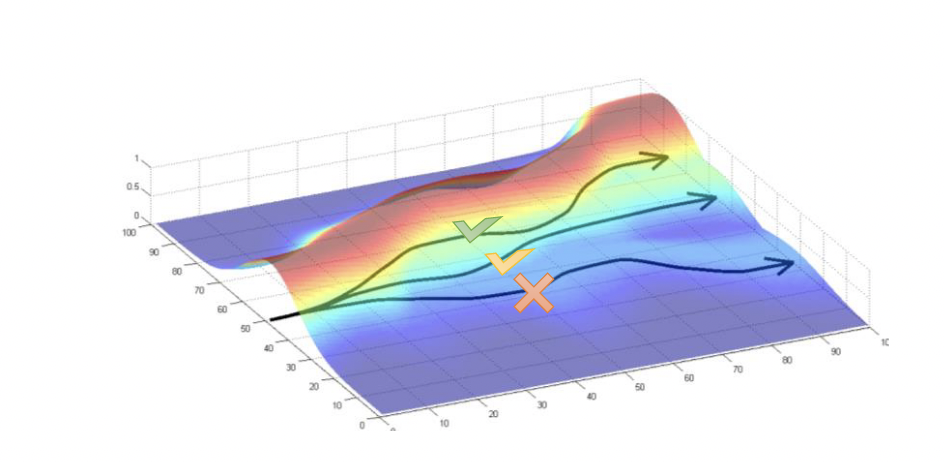
\includegraphics[scale=0.4]{loss_landscape.png}
	\caption{Paths across optimization landscape}
\end{figure*}\\
Using the REINFORCE Algorithm, we collect playouts at the beginning of each loop, so the value function of any state in the playout can be the actual reward-to go calulation, simply the sum of all future rewards following that observation. We may optionally specify a discount factor $\gamma$ for this calculation, however, in the case of sparse rewards, or uniform-dense rewards, it is almost always better to have a discount factor close to 1. 

\newpage
\nocite{*}
\bibliographystyle{apacite}{}
\bibliography{references}
	

\end{document}
